% Standalone source of the figure fig:interface: cells at a welded interface, in a vertical section.
% Build: pdflatex fig_interface.tex; the paper includes the PDF. Grey scale only.
% z is depth and points down; the interface is z = 0; medium A above, medium B below. Units of h, cell side 2.
% (a) Both cells in A, touching the interface and each other: the reflected coupling sees the source cell's
%     mirror image (dashed), which touches the field cell at the singular point.
% (b) A source cell in A and a field cell in B, touching at a point of the interface: the transmitted coupling.
\documentclass[border=2pt]{standalone}
% Shared preamble of the standalone figures of the interface paper.
\usepackage{amsmath,amssymb,bm}
\usepackage{tikz}
\usetikzlibrary{calc,arrows.meta}
\newcommand{\bR}{\mathbf{R}}
\newcommand{\bs}{\mathbf{s}}
\newcommand{\bu}{\mathbf{u}}
\newcommand{\bx}{\mathbf{x}}

\begin{document}
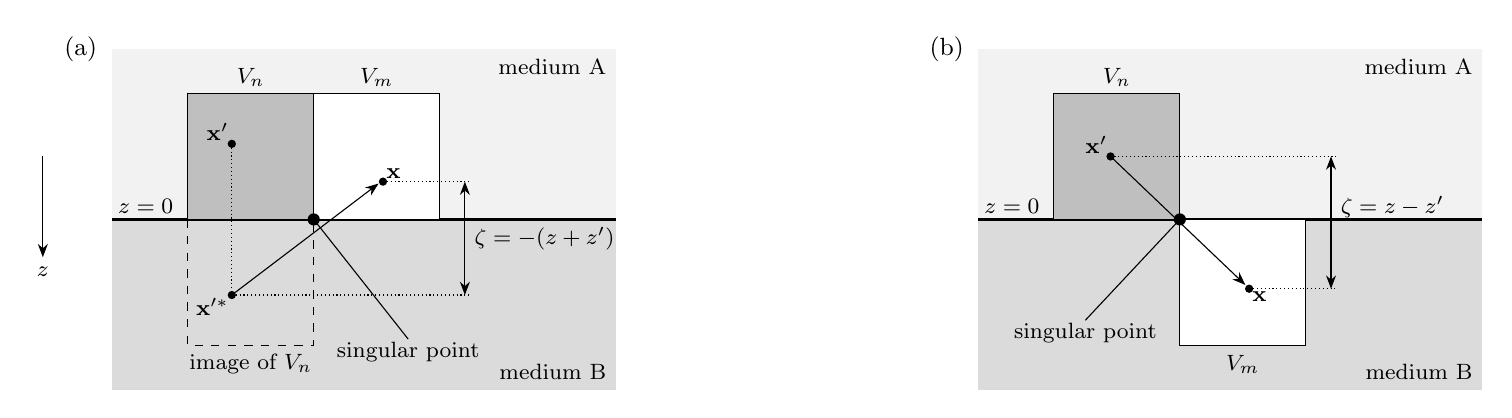
\begin{tikzpicture}[>=Stealth, x=0.8cm, y=0.8cm, font=\small]
  % tikz y = -z
  \newcommand{\panel}[1]{%
    \fill[black!5] (-1.2,0) rectangle (6.8,2.7);
    \fill[black!14] (-1.2,-2.7) rectangle (6.8,0);
    \draw[very thick] (-1.2,0) -- (6.8,0);
    \node[anchor=north east, font=\footnotesize] at (6.8,2.7) {medium A};
    \node[anchor=south east, font=\footnotesize] at (6.8,-2.7) {medium B};
    \node[anchor=south west, font=\footnotesize, inner sep=2pt] at (-1.2,0) {$z=0$};
    \node at (-1.7,2.7) {#1};
  }
  % ---------------------------------------------------------------- (a) reflection
  \begin{scope}
    \panel{(a)}
    \filldraw[fill=black!25, draw=black] (0,0) rectangle (2,2);
    \node[font=\footnotesize] at (1,2.25) {$V_n$};
    \filldraw[fill=white, draw=black] (2,0) rectangle (4,2);
    \node[font=\footnotesize] at (3,2.25) {$V_m$};
    \draw[dashed] (0,0) rectangle (2,-2);
    \node[font=\footnotesize] at (1,-2.3) {image of $V_n$};
    % a source point, its image, and a field point
    \fill (0.7,1.2) circle (1.5pt) node[above left, font=\footnotesize, inner sep=1pt] {$\mathbf x'$};
    \fill (0.7,-1.2) circle (1.5pt) node[below left, font=\footnotesize, inner sep=1pt] {$\mathbf x'^{*}$};
    \draw[densely dotted] (0.7,1.2) -- (0.7,-1.2);
    \fill (3.1,0.6) circle (1.5pt) node[above right, font=\footnotesize, inner sep=1pt] {$\mathbf x$};
    \draw[->, thin] (0.7,-1.2) -- (3.03,0.57);
    % zeta = -(z + z') is the depth of x' * below x
    \draw[<->, thin] (4.4,0.6) -- (4.4,-1.2);
    \draw[densely dotted] (3.1,0.6) -- (4.5,0.6) (0.7,-1.2) -- (4.5,-1.2);
    \node[right, font=\footnotesize] at (4.4,-0.3) {$\zeta=-(z+z')$};
    \fill (2,0) circle (2.2pt);
    \draw[thin] (2,0) -- (3.5,-1.9) node[below, font=\footnotesize, inner sep=1pt] {singular point};
  \end{scope}
  % ---------------------------------------------------------------- (b) transmission
  \begin{scope}[xshift=11.0cm]
    \panel{(b)}
    \filldraw[fill=black!25, draw=black] (0,0) rectangle (2,2);
    \node[font=\footnotesize] at (1,2.25) {$V_n$};
    \filldraw[fill=white, draw=black] (2,0) rectangle (4,-2);
    \node[font=\footnotesize] at (3,-2.3) {$V_m$};
    \fill (0.9,1.0) circle (1.5pt) node[above left, font=\footnotesize, inner sep=1pt] {$\mathbf x'$};
    \fill (3.1,-1.1) circle (1.5pt) node[below right, font=\footnotesize, inner sep=1pt] {$\mathbf x$};
    \draw[->, thin] (0.9,1.0) -- (3.04,-1.04);
    \draw[<->, thin] (4.4,1.0) -- (4.4,-1.1);
    \draw[densely dotted] (0.9,1.0) -- (4.5,1.0) (3.1,-1.1) -- (4.5,-1.1);
    \node[right, font=\footnotesize] at (4.4,0.2) {$\zeta=z-z'$};
    \fill (2,0) circle (2.2pt);
    \draw[thin] (2,0) -- (0.5,-1.6) node[below, font=\footnotesize, inner sep=1pt] {singular point};
  \end{scope}
  % depth axis
  \draw[->] (-2.3,1.0) -- (-2.3,-0.6) node[below, font=\footnotesize] {$z$};
\end{tikzpicture}
\end{document}
